\documentclass[11pt]{article}
\usepackage[a4paper,margin=1in]{geometry}
\usepackage{amsmath,amssymb}
\usepackage{graphicx}
\usepackage{booktabs}
\usepackage{float}
\usepackage{hyperref}

\title{Offline Coefficient-Space Comparison\\Full Data-Driven Maps (ANN151 vs GPR151)}
\author{Sebastian Ares de Parga Regalado}
\date{\today}

\begin{document}
\maketitle

\section*{Setup}
The two models compared here are full data-driven maps
\[
(\mu_1,\mu_2,t)\mapsto q_N(t;\mu)\in\mathbb{R}^{151},
\]
trained on Stage-2 PROM coefficients.

Reference trajectories are linear PROM coefficients $q_N^{lin}(t;\mu)$ at three verification points.
No online nonlinear ROM solve is used in this diagnostic.

\section*{Error definitions}
For each global coefficient $i=1,\dots,151$:
\[
E_i^{abs}(\mu)=\left\|q_i^{lin}-q_i^{pred}\right\|_2,\qquad
E_i^{rel}(\mu)=100\frac{\left\|q_i^{lin}-q_i^{pred}\right\|_2}{\left\|q_i^{lin}\right\|_2+\varepsilon}.
\]
Global trajectory error:
\[
E_F(\mu)=100\frac{\left\|Q^{lin}-Q^{pred}\right\|_F}{\left\|Q^{lin}\right\|_F+\varepsilon}.
\]

\section*{Pointwise summary (\%)}
\begin{table}[H]
\centering
\caption{Offline coefficient errors per point.}
\begin{tabular}{lccccc}
\toprule
Model & $\mu$ & $E_F$ & mean$(E_i^{rel})$ & p95$(E_i^{rel})$ & max$(E_i^{rel})$ \\
\midrule
ANN ns151 & (4.560,0.0190) & 3.842 & 49.200 & 101.068 & 118.742 \\
GPR ns151 & (4.560,0.0190) & 100.656 & 100.093 & 100.531 & 103.486 \\
\hline
ANN ns151 & (4.875,0.0225) & 1.791 & 30.688 & 79.297 & 87.480 \\
GPR ns151 & (4.875,0.0225) & 1.86e-05 & 2.87e-04 & 1.02e-03 & 1.36e-03 \\
\hline
ANN ns151 & (5.190,0.0260) & 5.474 & 53.547 & 105.780 & 138.958 \\
GPR ns151 & (5.190,0.0260) & 99.744 & 99.976 & 100.055 & 100.539 \\
\hline
\bottomrule
\end{tabular}
\end{table}

\section*{Average over the three points (\%)}
\begin{table}[H]
\centering
\caption{Average offline coefficient errors over the three points.}
\begin{tabular}{lcccc}
\toprule
Model & mean $E_F$ & mean(mean$(E_i^{rel})$) & mean(p95$(E_i^{rel})$) & mean(max$(E_i^{rel})$) \\
\midrule
ANN ns151 & 3.702 & 44.479 & 95.382 & 115.060 \\
GPR ns151 & 66.800 & 66.690 & 66.862 & 68.009 \\
\bottomrule
\end{tabular}
\end{table}

\section*{Per-coefficient curves}
\begin{figure}[H]
\centering
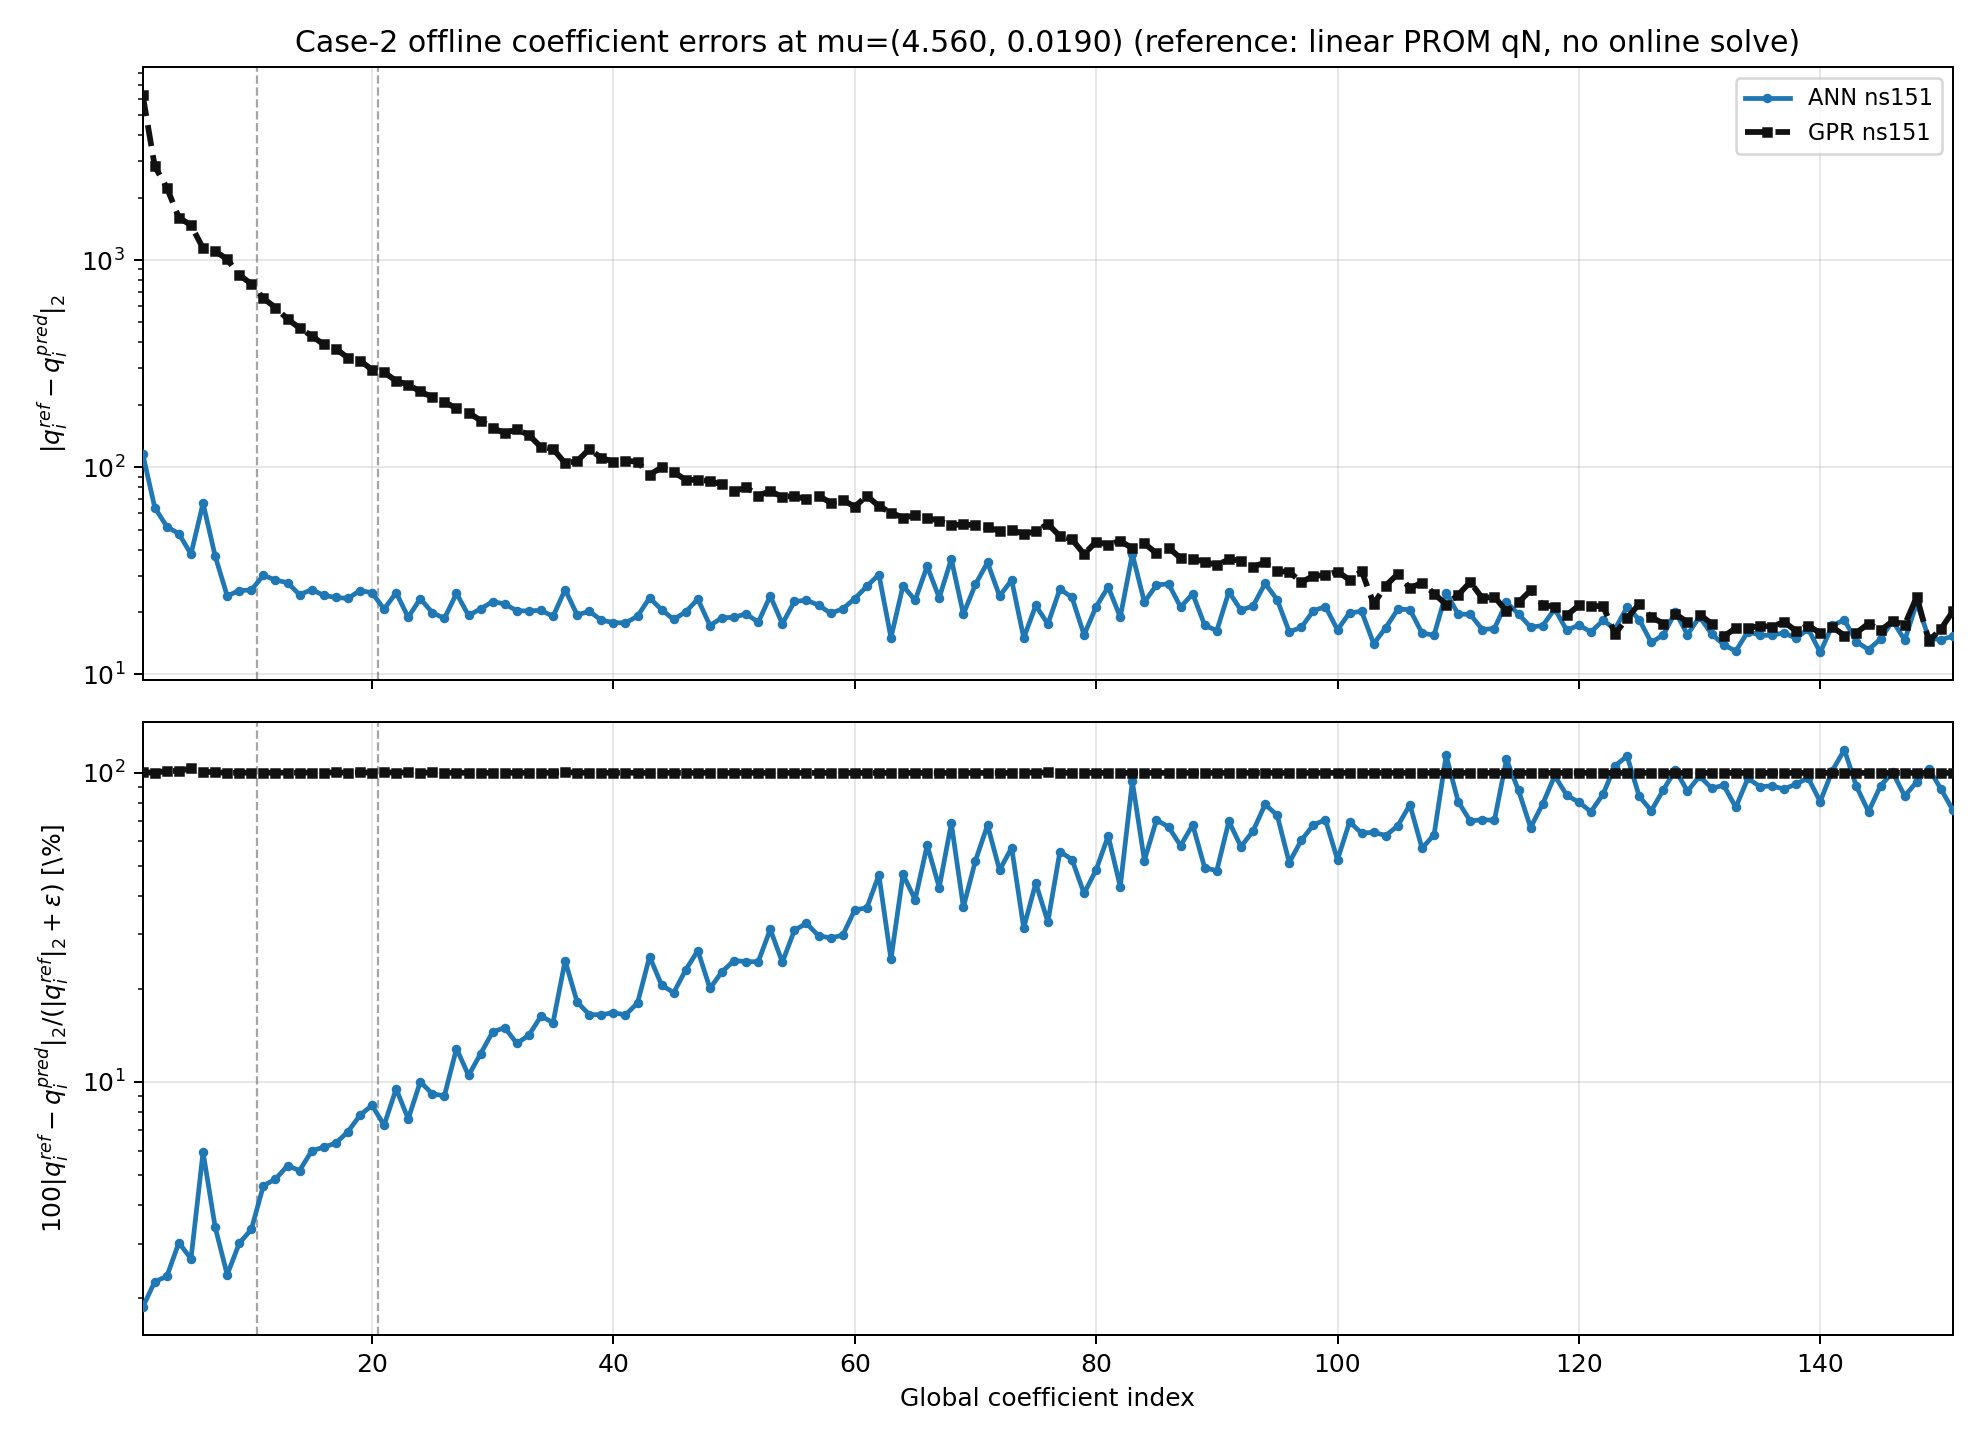
\includegraphics[width=0.96\textwidth]{Figures/data_driven151_coeff_offline/mu1_4.560_mu2_0.0190_coeff_abs_rel_vs_global_index_dd_ann_gpr_151.png}
\caption{Absolute and relative coefficient errors vs global coefficient index at $\mu^{(1)}=(4.560,0.0190)$.}
\end{figure}

\begin{figure}[H]
\centering
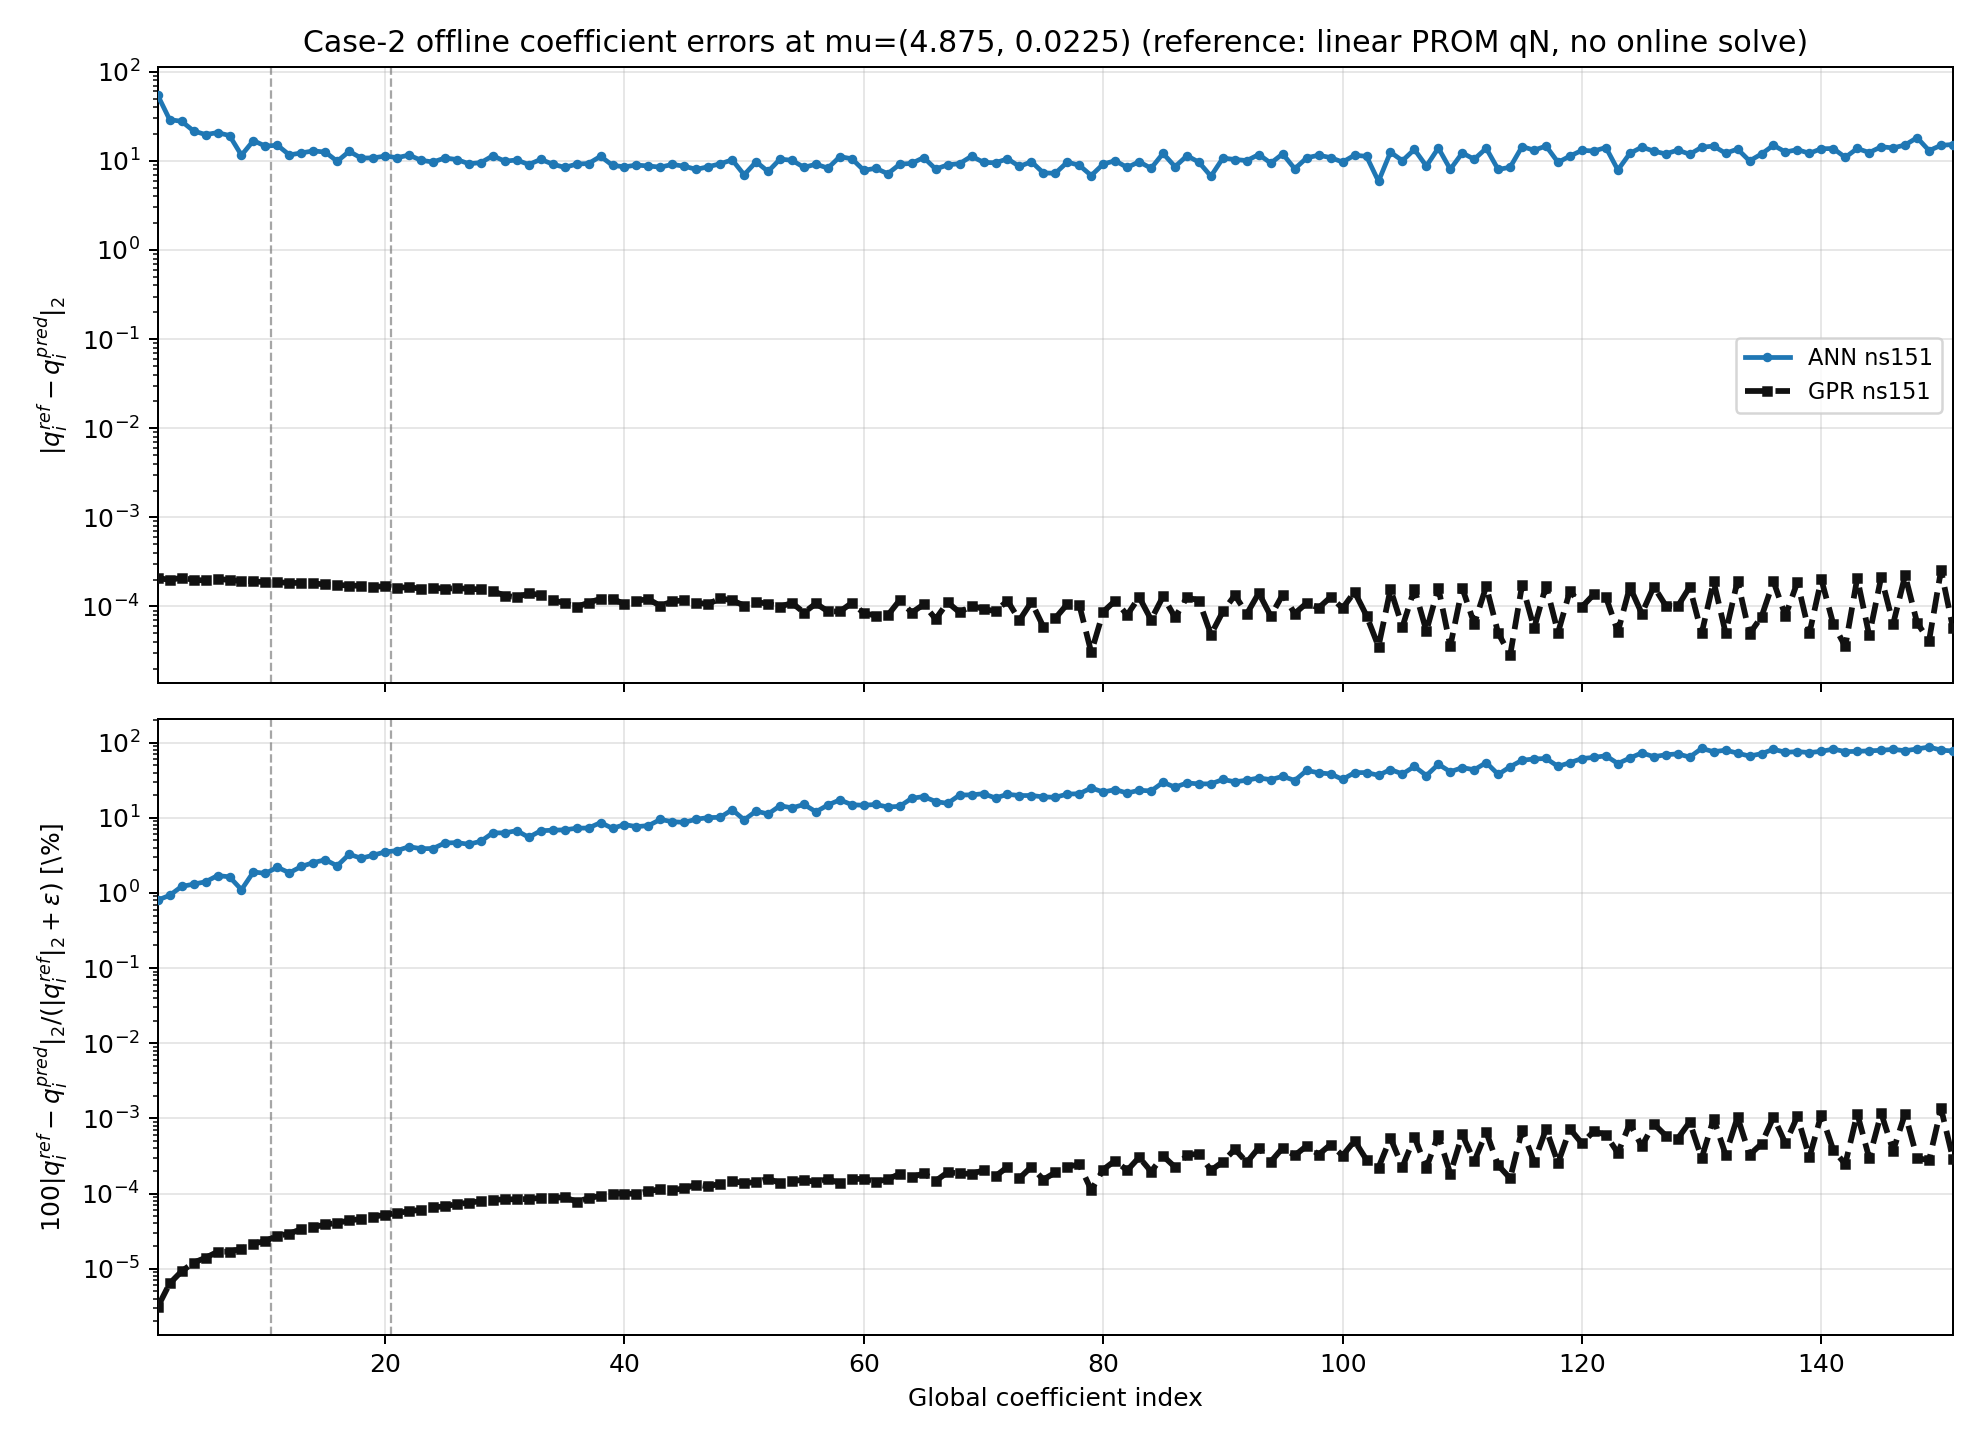
\includegraphics[width=0.96\textwidth]{Figures/data_driven151_coeff_offline/mu1_4.875_mu2_0.0225_coeff_abs_rel_vs_global_index_dd_ann_gpr_151.png}
\caption{Absolute and relative coefficient errors vs global coefficient index at $\mu^{(2)}=(4.875,0.0225)$.}
\end{figure}

\begin{figure}[H]
\centering
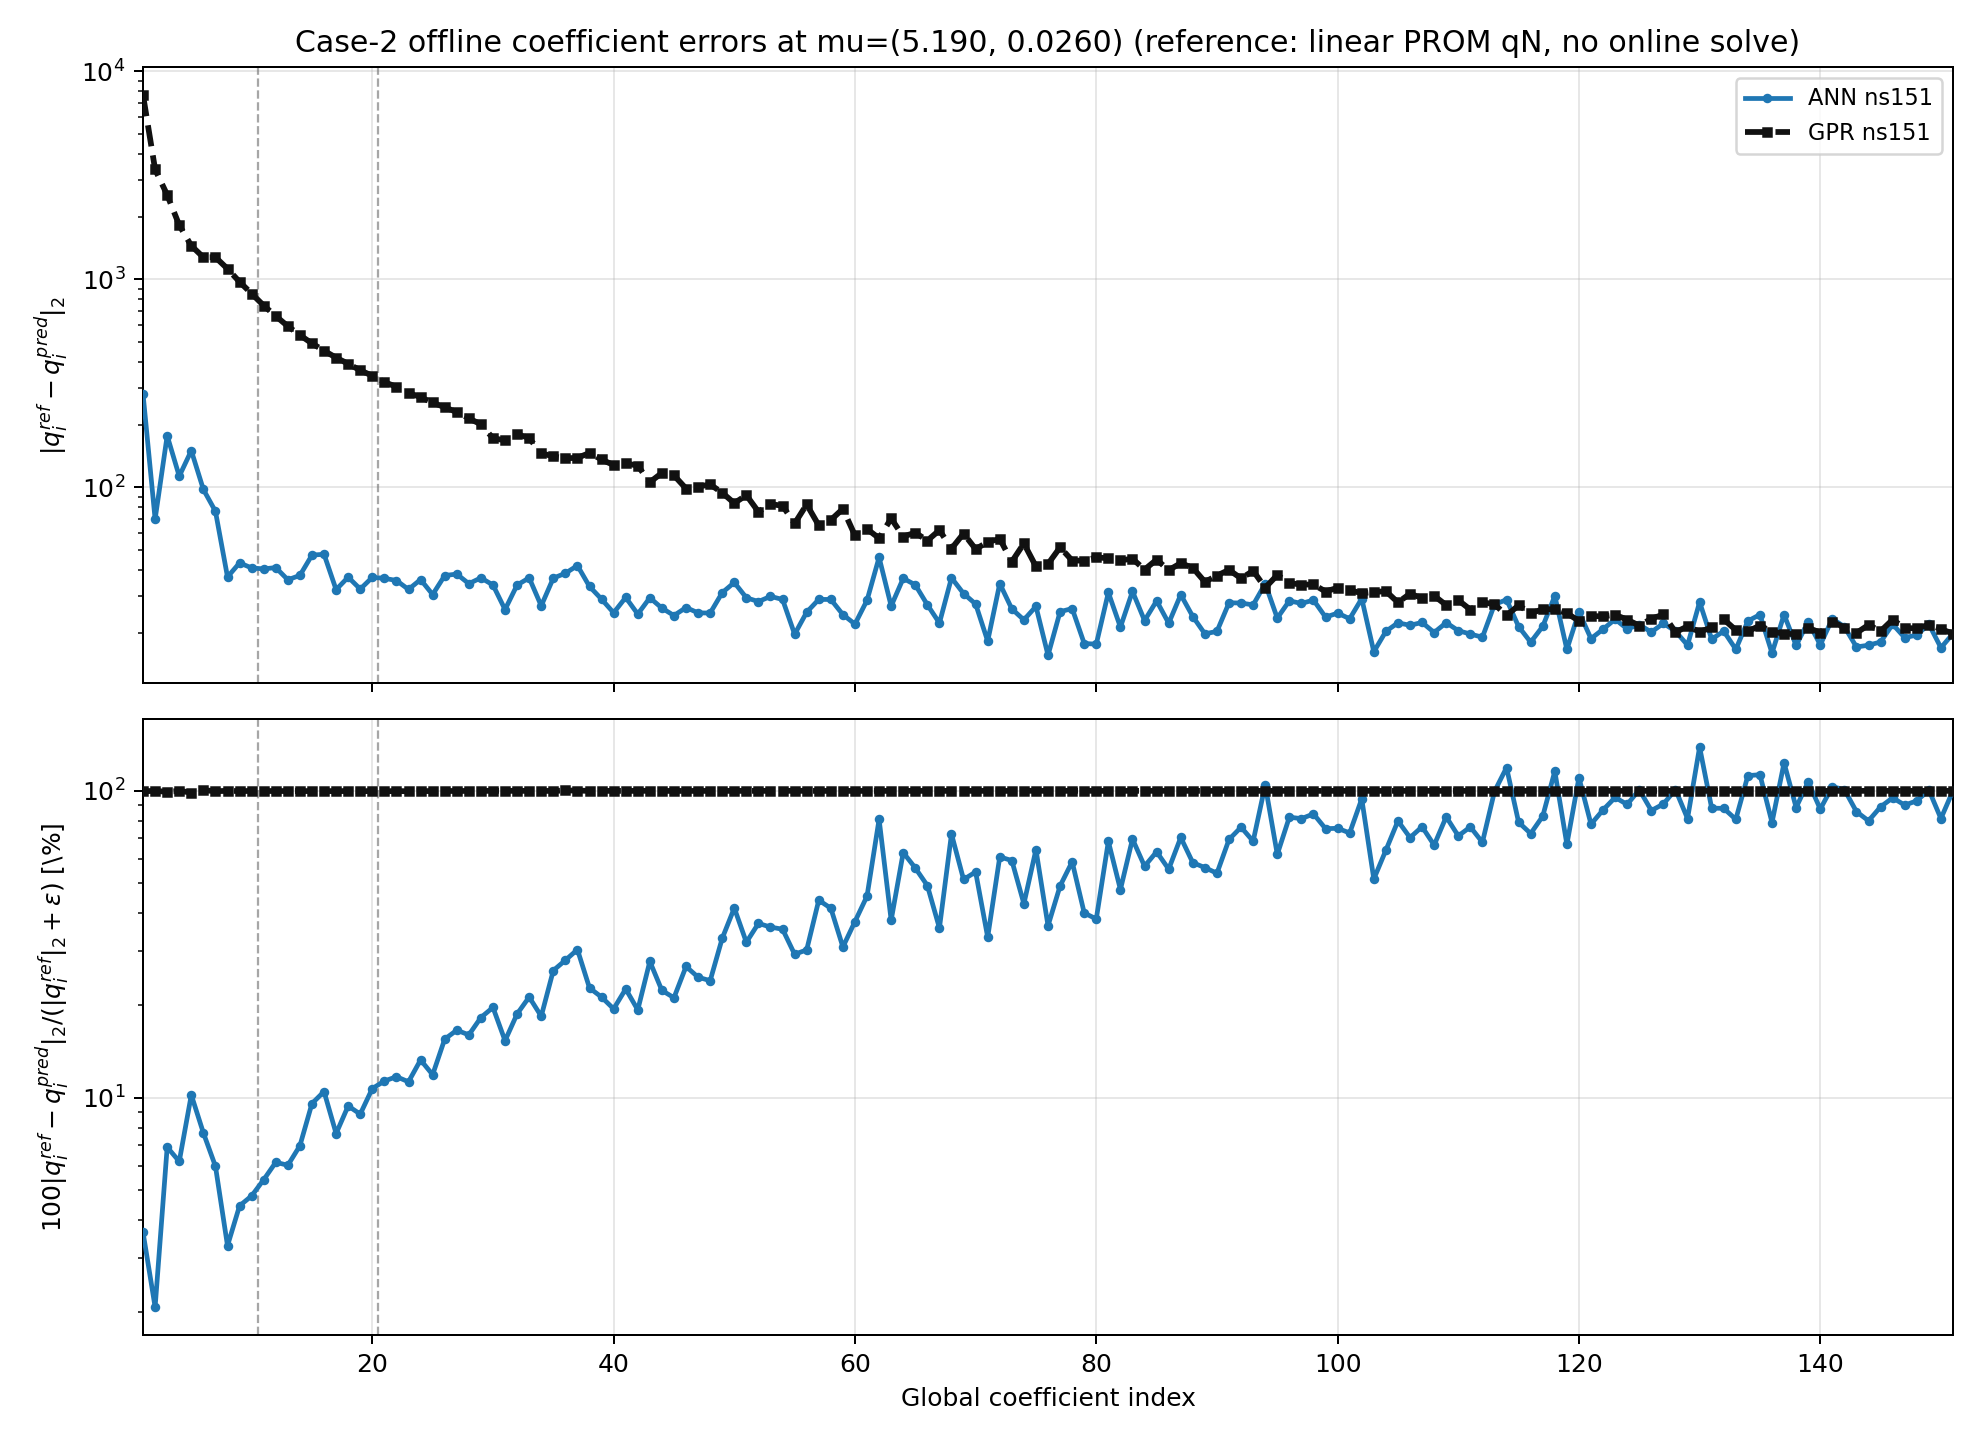
\includegraphics[width=0.96\textwidth]{Figures/data_driven151_coeff_offline/mu1_5.190_mu2_0.0260_coeff_abs_rel_vs_global_index_dd_ann_gpr_151.png}
\caption{Absolute and relative coefficient errors vs global coefficient index at $\mu^{(3)}=(5.190,0.0260)$.}
\end{figure}

\end{document}
